\documentclass[11pt]{article}

%\usepackage{palatino}

\usepackage[utf8]{inputenc}
\usepackage[T1]{fontenc}
% Chivo como en las diapositivas o Fira Sans?
%\usepackage[familydefault,regular]{Chivo}
\usepackage[sfdefault,scaled=.85]{FiraSans}
\usepackage{newtxsf}
\usepackage{mathastext}
\usepackage[spanish]{babel}
\setlength{\parindent}{0pt}
\usepackage{amssymb}
\usepackage{amsmath}
\usepackage{wasysym}
\usepackage[x11names, rgb, html]{xcolor}
\usepackage{graphics}
\usepackage{caption}
\usepackage{lipsum}
\usepackage{float}
\usepackage{adjustbox}
\usepackage{geometry}
\usepackage[scaled=.85]{FiraMono}
\usepackage{algpseudocode}
\usepackage{algorithm}
\usepackage{hyperref}

\hypersetup{
  % hidelinks = true,   % Oculta todos los enlaces.
  colorlinks = true,   % Muestra todos los enlaces, sin bordes alrededor.
  linkcolor={black},     % Color de enlaces genéricos
  citecolor={black},   % Color de enlaces de referencias
  urlcolor={blue!70!black}     % Color de enlaces de URL
}

\geometry{left=3cm,right=3cm,top=3cm,bottom=3cm,headheight=1cm,headsep=0.5cm}

%%% PGFPLOTSTABLE

\usepackage{pgfplotstable}

%%% COLORES

\definecolor{50}{HTML}{FFEBEE}
\definecolor{100}{HTML}{FFCDD2}
\definecolor{200}{HTML}{EF9A9A}
\definecolor{300}{HTML}{E57373}
\definecolor{400}{HTML}{EF5350}
\definecolor{500}{HTML}{F44336}
\definecolor{600}{HTML}{E53935}
\definecolor{700}{HTML}{D32F2F}
\definecolor{800}{HTML}{C62828}
\definecolor{900}{HTML}{B71C1C}



%% Colores de Solarized

\definecolor{sbase03}{HTML}{002B36}
\definecolor{sbase02}{HTML}{073642}
\definecolor{sbase01}{HTML}{586E75}
\definecolor{sbase00}{HTML}{657B83}
\definecolor{sbase0}{HTML}{839496}
\definecolor{sbase1}{HTML}{93A1A1}
\definecolor{sbase2}{HTML}{EEE8D5}
\definecolor{sbase3}{HTML}{FDF6E3}
\definecolor{syellow}{HTML}{B58900}
\definecolor{sorange}{HTML}{CB4B16}
\definecolor{sred}{HTML}{DC322F}
\definecolor{smagenta}{HTML}{D33682}
\definecolor{sviolet}{HTML}{6C71C4}
\definecolor{sblue}{HTML}{268BD2}
\definecolor{scyan}{HTML}{2AA198}
\definecolor{sgreen}{HTML}{859900}

%% Colores del documento

\definecolor{text}{RGB}{78,78,78}
\definecolor{accent}{RGB}{129, 26, 24}

%%% LISTINGS

\usepackage{listingsutf8}

%% Las tildes

\lstset{
  inputencoding=utf8/latin1
}

%% Colores de Solarized para listings

\lstset{
  % How/what to match
  % sensitive=true,
  % language=pseudo,
  % Border (above and below)
  frame=leftline,
  rulecolor=\color{300},
  framerule=2pt,
  % Line number
  numbers=left,
  % Extra margin on line (align with paragraph)
  xleftmargin=\parindent,
  % Put extra space under caption
  belowcaptionskip=1\baselineskip,
  % Colors
  % backgroundcolor=\color{sbase3},
  basicstyle=\footnotesize\ttfamily\color{sbase00},
  keywordstyle=\color{700},
  commentstyle=\color{300},
  stringstyle=\color{500},
  numberstyle=\color{500},
  %identifierstyle=\color{500},
  % Break long lines into multiple lines?
  breaklines=true,
  % Show a character for spaces?
  showstringspaces=false,
  tabsize=2,
  xleftmargin=0.7em,
}

\renewcommand{\lstlistingname}{Código fuente}% Listing -> Algorithm


\title{Algorítmica: práctica 4 \\ \large El recorrido del caballo\\ \vspace{0.2em}Grupo 2}
\author{Sofía Almeida Bruno \and Antonio Coín Castro \and María Victoria Granados Pozo \and Miguel Lentisco Ballesteros \and José María Martín Luque}
\date{\today}

\begin{document}
\maketitle

\newpage

\section*{Análisis del problema}

Dado un tablero de ajedrez de tamaño $N\times N$ y un caballo colocado en una posición inicial, nuestro problema consiste en pasar por todas las casillas del tablero una sola vez realizando los movimientos permitidos para el caballo. Coloquialmente, se conoce como el \textbf{problema del recorrido del caballo.}

\begin{figure}[H]
  \centering
  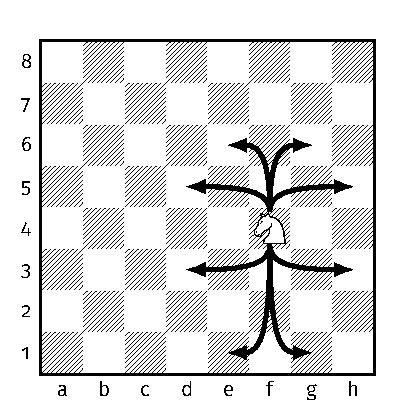
\includegraphics{./img/tablero1.pdf}
  \caption{Movimientos posibles del caballo}
  \label{}
\end{figure}

Antes de comenzar con el diseño de un algoritmo que resuelva el problema, hemos consultado algunos artículos donde se discute el mismo. Por ejemplo, \textit{Cull et al.} \cite{cull} probaron el siguiente resultado:\\

\textbf{Teorema.} \textit{Todo tablero de tamaño $N\times M$ con $	min(N,M)\ge5$ tiene un recorrido válido del caballo.}\\

Además, consultando la secuencia \cite{sequence}, observamos que el problema no tiene solución en un tablero $N\times N$ si $N=2,3,4$. El caso $N=1$ se considera trivial, por lo que pondremos especial hincapié en el caso $N\ge5$.\\

Para representar nuestro problema, hemos usado una clase \verb|TableroAjedrez|. En \verb|TableroAjedrez| se encapsula la matriz que simboliza un tablero de ajedrez de tamaño $N\times N$, hasta un máximo fijado. Además, disponemos de un \verb|struct Posicion| que representa una casilla del tablero, para poder gestionar los posibles desplazamientos del caballo. Se adjunta el código fuente de la clase.\\

La solución es una secuencia de pasos que reflejan el movimiento del caballo a lo largo del tablero. A la hora de representarlo, modificaremos directamente el tablero, considerando que el contenido de la posición \verb|(i,j)| es el paso en el que el caballo se situó en la casilla que representa dicha posición. Inicialmente, todas las casillas del tablero contienen un $0$.

\section*{Técnica utilizada}

Notemos que podemos representar nuestro problema utilizando un grafo, en particular, un árbol de estados, donde los nodos serían los tableros con las posibles posiciones del caballo en cada paso. La raíz sería un tablero con la posición inicial, que en cada nivel se va ramificando para permitirnos considerar todas las opciones de desplazamiento disponibles. De las dos técnicas estudiadas para exploración de grafos hemos utilizado \textit{BackTracking} porque consideramos que se adapta mejor al problema que nos enfrentamos.\\

\textit{Branch\&Bound} es un procedimiento enfocado a resolver problemas de optimización, ya que se aprovecha del uso de cotas. En este caso, como simplemente queremos llegar a una solución sin minimizar ni maximizar ninguna función objetivo, no necesitamos esta técnica.

\begin{figure}[h]
  \centering
  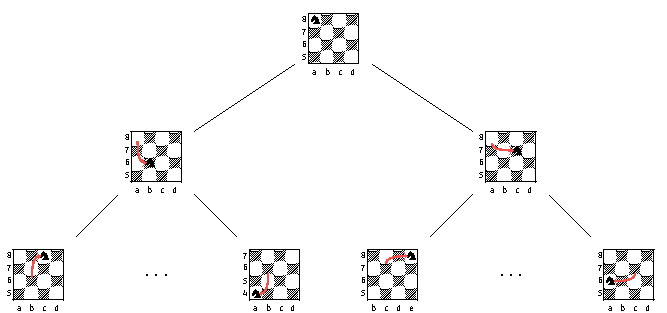
\includegraphics[scale=1.8]{img/arbol-estados.pdf}
\caption{Representación simplificada del árbol de estados} \label{fig:árbol}
\end{figure}

En la representación del árbol de estados, cada nodo tendría 8 hijos (tantos como posibles movimientos del caballo), pero solo se ven el primero y el último por cuestiones de espacio. Además, el problema en su versión más conocida se enuncia en un tablero de $8\times 8$, que tampoco se muestra completo en los nodos por el mismo problema de espacio.

\section*{Diseño de la solución}

Empleando un enfoque basado en la técnica \textit{BackTracking} para la resolución del problema, la idea es la siguiente: partiendo del tablero inicial exploraremos todos los tableros de movimientos posibles, y cada uno de ellos en profundidad. Finalizaremos cuando en alguno nos devuelva una solución.\\

Vamos a mostrar las componentes \textit{BackTracking} de este problema:

\begin{itemize}
	\item \textit{Representación de la solución:} una matriz de enteros $M=(m_{ij})$ donde cada entrada representa el paso en el que el caballo se situó en la posición (i,j).
	\item \textit{Restricciones implícitas:} el número de paso añadido tiene que ser menor o igual que $N^2$, donde $N$ es la dimensión del tablero.
	\item \textit{Restricciones explícitas:} el caballo no puede salirse del tablero ni situarse en una casilla por la que ya se ha pasado. Además, solo puede realizar movimientos válidos según las reglas del ajedrez.
	\item \textit{Función objetivo:} encontrar un tablero en el que el caballo se ha desplazado por todas las casillas una única vez.
	\item \textit{Función de poda:} un nodo será explorado si cumple: el caballo no se sale del tablero (la posición no supera el tamaño de la matriz para ninguna de sus componentes), y además no ocupa una casilla por la que se ha pasado (el valor de dicha casilla es diferente de $0$, valor al que se inicializan todas las casillas del tablero).
	\item \textit{Representación del árbol implícito:} en cada nivel $i$ del árbol asignamos cada una de las posibles posiciones del caballo en el paso $i$-ésimo. Este árbol es el que muestra la Figura \ref{fig:árbol}.
\end{itemize}

Una vez que hemos visto las componentes, pasemos a ver un esqueleto o \textit{pseudocódigo} del algoritmo: \\

$Tablero[1,\dots,N][1,\dots,N] \equiv \text{ Representa el tablero. Tras finalizar, representa la solución}\\ N \equiv \text{ Dimensión del tablero }\\ pos \equiv \text{ Posición actual del caballo $(i,j)$ en el tablero}\\ k \equiv \text{ Paso actual}$\\

\begin{algorithm}[H]
\begin{algorithmic}

\Function{MovimientosCaballoBT }{$Tablero[1,\dots,N][1,\dots,N]$, pos, $k$}
     \State $Tablero[pos] \gets k$ \Comment Casilla elegida

     \If{$k == n^2$} \Comment Hay solución
     	\State \Return true
    	\EndIf
     \For{mov $in$ \textit{Movimientos válidos del caballo}}
         \State $pos \gets pos + mov$
         \If{esFactible(mov)} \Comment Función de poda
         	\State correcto $\gets$ MovimientosCaballoBT(Tablero, pos, $k+1$) \Comment 						Explora siguiente nivel
         	\If{correcto}
         		\State \Return true
         	\Else
         		\State $Tablero[pos] \gets 0$ \Comment Movimiento sin solución
         	\EndIf
         \EndIf
      \EndFor
     \State \Return false \Comment  Sin solución en pasos siguientes
  \EndFunction
\end{algorithmic}
\end{algorithm}

Observamos que necesitamos una estructura de datos adicional, donde se almacenen los \textit{movimientos válidos del caballo}. Dichos movimientos serán relativos a la posición que en ese momento ocupe el caballo, es decir, si la posición actual es $(i,j)$, los movimientos válidos son alguno de $(i \pm 2, j \pm 1)$ ó $(i \pm 1, j \pm 2)$.\\

En la práctica, hemos implementado las \textit{restricciones implícitas} como una comprobación para saber si se ha llegado a una solución, pues, por la construcción del algoritmo, cuando se llegue a $N^2$ pasos, se habrá conseguido la \textit{función objetivo}. Además, la \textit{función de poda} se ha separado y renombrado por simplicidad.

\section*{Algoritmo BackTracking}

Veamos ahora el algoritmo implementado en el lenguaje \verb|C++|. En primer lugar, hemos separado la implementación de la \textit{función de poda}, para que se aprecie con claridad. Su funcionalidad es la que se describió anteriormente.

	\lstinputlisting[language=C++, linerange={19-24}, caption=Criterio de Factibilidad]{./../src/Algoritmo.cpp}
\vspace{1em}

Ahora pasemos a la función principal. En primer lugar, se coloca en la casilla actual el número de paso que se recibe como argumento. A continuación, el algoritmo comprueba si está en el último paso, pues de ser así habrá encontrado solución y terminará, devolviendo \textbf{true}.\\

En caso contrario, el algoritmo se repetirá con cada una de las casillas a las que puede moverse el caballo desde la posición en la que se encuentra (cumpliendo las restricciones consideradas anteriormente), y aumentando en $1$ el paso. Dichas posiciones se encuentran en un vector y se irán sumando a la posición actual para ir calculando las nuevas. Se comprueba si las posiciones son factibles con la función anteriormente mostrada.\\

	\lstinputlisting[language=C++, linerange={15-16}, caption=Vector de movimientos válidos del caballo]{./../src/Algoritmo.cpp}
	\vspace{1em}


Al realizar la llamada recursiva, esta puede devolver \textit{true} o \textit{false}. En el primer caso, significaría que en el nivel siguiente se  ha permitido seguir avanzando (o se ha llegado al final), por lo que el algoritmo finaliza devolviendo \textbf{true}. En el segundo caso, la razón sería que en el siguiente nivel no se ha encontrado ninguna posición válida para colocar el caballo. Entonces, tenemos que volver a poner a $0$ la casilla por la que hemos intentado pasar, y continuar con el siguiente movimiento. En caso de que ningún movimiento sea válido, devolveremos \textbf{false}.\\

El algoritmo continúa repitiendo el paso anterior hasta que se haya pasado por todas las posiciones del tablero (notemos que no volverá a seleccionar nunca una casilla ya considerada). Cuando finalice, tendremos como solución una matriz donde cada casilla contiene el número de paso del caballo.\\


\lstinputlisting[language=C++, linerange={26-49}, caption=Algoritmo BackTracking]{./../src/Algoritmo.cpp}

Por último, comentaremos el programa principal \verb|main|, donde diferenciamos varios casos:
\begin{itemize}
	\item Si no se pasa como parámetro la posición inicial generaremos una posición aleatoria hasta que encontremos una solución al problema. Este proceso, en general, puede ser muy costoso, pues como veremos la eficiencia del algoritmo para una posición dada es ya exponencial. La primera posición a comprobar será la $(0,0)$, pues es más probable que empezando en una esquina encontremos una solución.
	\item Si el tamaño del tablero menor que $5x5$ nunca se obtendrá una solución, por tanto solo se ejecutará el algoritmo si $N\ge5$. Sin embargo, si lo ejecutásemos nos devolvería correctamente que no hay solución. Si el tamaño es $1$, la solución (trivial) será la única casilla del tablero.
\end{itemize}


\section*{Ejemplo paso a paso}

%%% TODO: completar. Considerar hacer el ejemplo para un tamaño pequeño, digamos 5x5, y realizar el primer nivel y la primera vuelta atrás, suponiendo que no encuentra la solución. Suponer que en el segundo movimiento ya la encuentra.

Supongamos que llamamos a nuestro  programa pasándole como parámetro un 5, que indicará el número de filas y columnas. Así, tendremos un tablero de tamaño $5\times5$ cuyos elementos están inicializado a 0. Como no pasamos ningún otro argumento al ejecutar el programa la posición inicial será la (0,0).\\

\begin{figure}[H]
  \centering
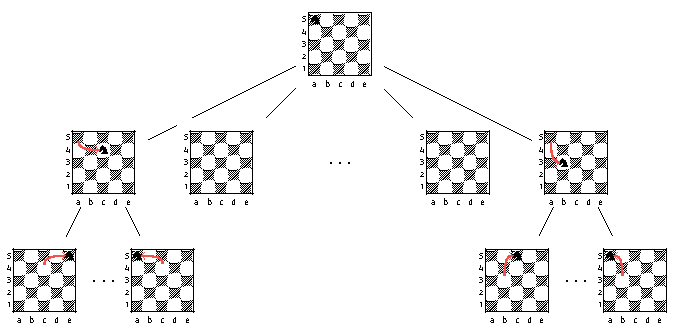
\includegraphics[scale=1.3]{img/arbol-ejemplo.pdf}
\caption{Representación simplificada del árbol de estados del ejemplo} \label{fig:árbol-ejemplo}
\end{figure}

Invocamos el procedimiento BackTracking pasándole como parámetros el tablero ya inicializado, y por referencia (para evitar el elevado coste que provocaría la copia, ya que llamaremos recursivamente a este procedimiento); la posición inicial; y 1 como número de paso.\\

Lo primero que se hace es actualizar el contenido de la posición pasada al número de paso correspondiente. Nuestro tablero tendría entonces un 1 en la posición (0,0) y el resto continuaría a 0.
Se comprueba si estamos en el último paso y, como no lo estamos, continuamos con la ejecución de un bucle \verb|for| en el que se irán explorando los movimientos que puede realizar el caballo. La posición nueva será $(0,0)+$\verb|movimientos[0]|$=(0,0)+(2,1)$, donde \verb|movimientos| es el vector que almacena las posibles opciones de desplazamiento del caballo. Como esta posición se encuentra en el tablero y además no se ha pasado por ella, se cumple la condición para volver a llamar a la función BackTracking donde el paso será 2 e irá realizando el mismo algoritmo de forma recursiva. Una vez resuelta la recursividad, la función devolverá \textit{true} o \textit{false}.\\

Si devuelve \textit{true} es porque ya ha finalizado, es decir, se han ido produciendo las sucesivas llamadas al algoritmo hasta llegar al paso $N^2 = 25$, y se ha encontrado una solución. Pero si devuelve \textit{false} es porque a partir de la casilla actual no existe una solución para el movimiento elegido, por lo que volvemos a poner a 0 su contenido (dicho contenido cambió al llamar a la función para esta casilla). Continúa con la ejecución del bucle actualizando la posición a la siguiente que haya en el vector, es decir, $(0,0)+$\verb|movimientos[1]|, y ejecutando el mismo algoritmo otra vez para el paso 2.\\

Este proceso se repite hasta que el algoritmo finalmente encuentre una solución, que sabemos que ocurre siempre si $N\ge5$, por lo que en este caso sí la encontrará.


\section*{Eficiencia teórica}

Queremos hallar la eficiencia teórica de nuestro algoritmo en el peor de los casos. Esto ocurrirá cuando para llegar a la solución tengamos que recorrer el árbol implícito por completo. Dado que hay 8 movimientos del caballo posibles, en cada nivel el número de nodos se multiplica por 8 con respecto al nivel anterior. Seguiremos añadiendo niveles hasta que el tablero esté completo, es decir, hayamos recorrido las $N \times N$ casillas.\\

Por tanto, el número total de nodos que habría que recorrer sería la suma de los nodos de cada nivel, que podemos expresar como:
\begin{equation} \label{geo}
1 + 8 + 8^2 + \hdots + 8^{N^2} = \sum_{i=0}^{N^2} 8^i = \frac{8^{N^2} - 1}{8 - 1}
\end{equation}

Como en cada nodo únicamente realizamos una serie de operaciones con eficiencia constante, afirmamos que la eficiencia del algoritmo es de orden $O\left( 8^{N^2} \right)$. En particular, para un tablero estándar de ajedrez, el orden de eficiencia es: $$ O(8^{64}) = O(6.277 \cdot 10^{57} )$$

Esta eficiencia exponencial la hemos comprobado en múltiples ocasiones a la hora de ejecutar el algoritmo, ya que aunque funciona correctamente, no da una solución en un tiempo razonable para todas las posiciones iniciales.\\

Otra forma de analizar la eficiencia teórica sería resolver la ecuación en recurrencia: $$\begin{cases} T(1) = 1\\
                             T(N) = 8T(N-1)
\end{cases}$$ pues en cada paso se realizan como mucho, $8$ llamadas recursivas, donde habría una casilla menos por rellenar. Esta ecuación en recurrencia no es sino otra forma de expresar la progresión geométrica \eqref{geo}, ya que en cada paso se multiplica por un término constante, concretamente $8$, que es la razón de la progresión.

\section*{Problema real}

El problema del recorrido del caballo es un caso particular de un problema más general: hallar, si existe, un camino hamiltoniano \cite{wiki} en un grafo. Si además imponemos que desde la casilla donde finaliza el caballo se pueda volver a la casilla de origen mediante un movimiento válido, el problema se transforma en hallar un camino cerrado o ciclo hamiltoniano \cite{wiki}.\\

No se nos ocurre ninguna situación real de aplicación del problema del recorrido del caballo, tal y como lo hemos enunciado. Sin embargo, si consideramos el problema de hallar un camino cerrado, existe una similitud con el problema del \textit{viajante de comercio}, que consiste en hallar un ciclo hamiltoniano \textbf{minimal} para un grafo completo, no dirigido y ponderado.\\

\section*{Compilación y ejecución del proyecto}
Para compilar este proyecto simplemente hay que situarse en la carpeta \verb|p4_backtracking| y ejecutar el comando \verb|make|.\\

Una vez compilado, si estamos situados en la misma carpeta ejecutamos \verb|./bin/main| pasando como parámetro el tamaño del tablero, y opcionalmente la posición inicial del caballo. Un ejemplo del formato completo sería el siguiente: \verb|./bin/main 8 0 0|.\\

Si $N$ es el tamaño del tablero, las posiciones del caballo comienzan en $0$ y acaban en $N-1$, tanto para las filas como para las columnas.

% --------------------------------------------------------------------------------
% Bibliografía.
% --------------------------------------------------------------------------------
\begin{thebibliography}{9}

\bibitem{cull}
  Paul Cull, Jeffery De Curtins.
  \emph{Knight's tour revisited}.
   \href{http://www.fq.math.ca/Scanned/16-3/cull.pdf}{PDF}.

\bibitem{sequence}
  Sequence
  \href{https://oeis.org/A165134}{A165134} in the OEIS.

\bibitem{wiki}
  \href{https://en.wikipedia.org/wiki/Hamiltonian_path_problem}{Hamiltonian path problem} on Wikipedia.

\end{thebibliography}


\end{document}
